\begin{center}
	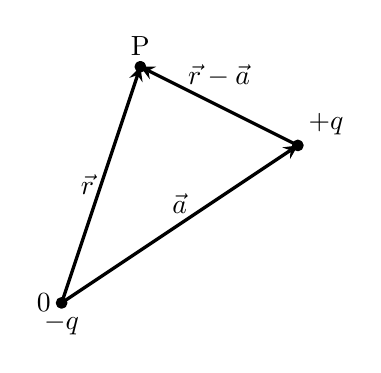
\begin{tikzpicture}[line width = 1.2pt, line join=round,x=1cm,y=1cm,>=stealth]
		% Achsen
		%\draw [->,dashed] (0,0) -- (4,0) node[anchor=north west] {$x$};
		%\draw [->,dashed] (0,0) -- (0,4) node[anchor=south east] {$y$};
		\draw (0,0) node[anchor=east] {$0$};
		% Koordinaten für die Ladungen
		\coordinate (a) at (0,0);
		\coordinate (b) at (3,2);
		% Koordinaten für den Raumpunkt
		\coordinate (c) at (1,3);
		% Vektor a
		\draw [->,color=black] (a) -- (b);
		\draw [color=black] (1.5,1) node[anchor = south] {$\vec{a}$};
		% Vektor r
		\draw [->,color=black] (0,0) -- (c);
		\draw [color=black] (0.55,1.5) node [anchor=east] {$\vec{r} $};
		% Vektor r-a
		\draw [->,color=black] (b) -- (c);
		\draw [color=black] (2,2.6) node[anchor=south] {$\vec{r}  - \vec{a}$};
		% partielle Ladungen
		\filldraw [color=black] (a) circle (1.5pt);
		\draw [color=black] (a) node[anchor=north] {$-q$};
		\filldraw [color=black] (b) circle (1.5pt);
		\draw [color=black] (b) node[anchor=south west] {$+q$};
		% Beobachtungspunkt
		\filldraw [color=black] (c) circle (1.5pt);
		\draw [color=black] (c) node[anchor= south] {$\mathrm{P} $};
	\end{tikzpicture}
\end{center}